\documentclass[UTF8]{ctexart}

\usepackage{amsmath}
\usepackage{listings}
\usepackage{tikz}

\title{Algorithms Homework 4}
\author{PB22111620 Ai Chang}

\begin{document}
\begin{sloppypar}

\maketitle

\section*{Q1}
    \subsection*{(a)}
        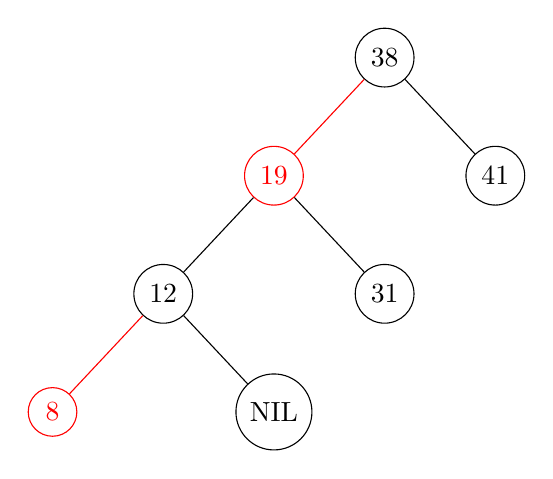
\begin{tikzpicture}[circle, sibling distance=80pt]
            \node[draw] [black]{38}
                child [red]{node[draw] [red]{19}
                    child [black]{node[draw] {12}
                        child [red]{node[draw] [red]{8}}
                        child [black]{node[draw] [black]{NIL}}
                    }
                    child [black]{node[draw] {31}}}
                child [black]{node[draw] {41}}
            ;
        \end{tikzpicture}
    \subsection*{(b)}
        \begin{enumerate}
            \item delete 8:

                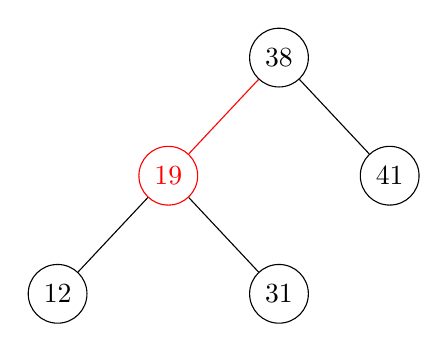
\begin{tikzpicture}[circle, sibling distance=80pt]
                    \node[draw] [black]{38}
                        child [red]{node[draw] [red]{19}
                            child [black]{node[draw] [black]{12}}
                            child [black]{node[draw] [black]{31}}
                        }
                        child [black]{node[draw] [black]{41}}
                    ;
                \end{tikzpicture}

            \item delete 12:

                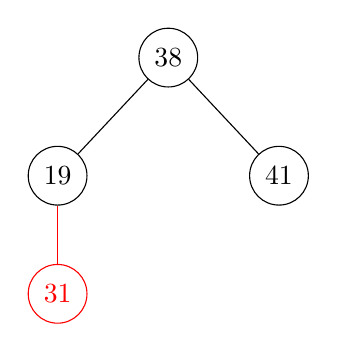
\begin{tikzpicture}[circle, sibling distance=80pt]
                    \node[draw] [black]{38}
                        child [black]{node[draw] [black]{19}
                            child [red]{node[draw] [red]{31}}
                        }
                        child [black]{node[draw] [black]{41}}
                    ;
                \end{tikzpicture}
            \item delete 19:

                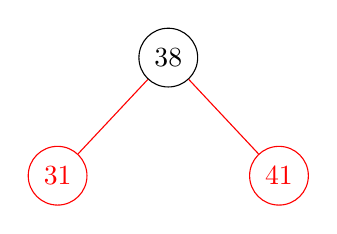
\begin{tikzpicture}[circle, sibling distance=80pt]
                    \node[draw] [black]{38}
                        child [red]{node[draw] [red]{31}}
                        child [red]{node[draw] [red]{41}}
                    ;
                \end{tikzpicture}
            \item delete 31:

                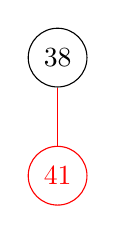
\begin{tikzpicture}[circle, sibling distance=80pt]
                    \node[draw] [black]{38}
                        child [red]{node[draw] [red]{41}}
                    ;
                \end{tikzpicture}
            \item delete 38:

                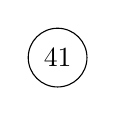
\begin{tikzpicture}[circle, sibling distance=80pt]
                    \node[draw] [black]{41}
                ;
                \end{tikzpicture}
            \item delete 41:

                
\begin{tikzpicture}[circle, sibling distance=80pt]
                    \node[draw] [black]{NIL};
                \end{tikzpicture}
        \end{enumerate}

\section*{Q2}
    \begin{enumerate}
        \item 黑高为 h 的红黑树内部节点最多有 $2^{2k} - 1$ 个, 理由如下:

            根据黑高的定义, 从根节点到 NIL 的任何一条路径上都有 k 个黑色节点, 根据红黑
            树的特点, 易知一条从根节点到 NIL 的路径上最多有 k 个红色节点. 当内部节点最
            多时, 每条路径均由黑、红节点交错组成. 若设根的深度为1, 则该红黑树为深度为 $2k$ 的满二叉树(不包括叶子节点所
            在层). 故内部节点总数为 $$N = 2^0 + 2^1 + \cdots + 2^{2k-1} = 2^{2k
            } - 1$$
        \item 内部节点最少有 $2^k - 1$ 个, 理由如下:

            与 1 类似, 当红黑树完全没有红色节点时, 内部节点最少, 此时红黑树为由黑色节点组
            成的深度为 k 的满二叉树.故内部节点个数为 $$N = 2^0 + 2^1 + \cdots + 2^{k-1}
            = 2^k - 1$$
    \end{enumerate}

\section*{Q3}
    \subsection*{(a)}
        (本题中的区间应专指闭区间,否则结论不成立. eg: 区间集合 A = {[0, 3], (1, 2)},
         最大重叠点包括 (1, 2) 中的所有点, 但其中没有区间端点)

        证明:假设所有的最大重叠点均不是任何一个区间的端点. 设其中一个最大重叠点为 x, 覆盖
        x 的所有区间为 \[[a_1, b_1], [a_2, b_2], \ldots, [a_n, b_n]\]
        则有 \[a_1, a_2, \ldots, a_n < x < b_1, b_2, \ldots, b_n\]
        取 \[b = min\{b_1, \ldots, b_n\}\]
        则 \[b \in [a_1, b_1], \ldots, [a_n, b_n]\]
        故覆盖 b 与覆盖 x 的区间数相同. 因为 x 是最大重叠点, 故 b 也是最大重叠点,
        且 b 是其中一个区间的端点.

        综上, 在最大重叠点中, 一定存在一个点是其中一个区间的端点.
    \subsection*{(b)}
        所设计的数据结构有误, 等待正确答案.
        所设计的数据结构如下:

        将红黑树进行修改, 每个节点额外存储三个值: int num, int value, int sum; 其中
        num 为 key-value, 对应一个区间端点的值, 若为左端点, value 设为 1, 否则设为 -1,
        对于端点 x, x.sum = x.left->sum + x.right->sum + x.value.

        INSERT-INTERVAL: 利用红黑树的操作插入操作分别插入两个端点值, 但在插入时, 如遇到
        x.num = node.num, 只需 node.value += x.value, node.sum += x.value. 然后
        自 node 向上维护各节点的 sum 值

        DELETE-INTERVAL: 执行 node.value

\section*{Q4}
    \subsection*{(a)}
        没有问题,在将节点 x 的孩子节点都加入 H 的根节点序列后, 移除 x 只需要修改 x 两侧
        节点的指针, 该操作的时间复杂度为 O(1)
    \subsection*{(b)}
        若 `$y \neq NIL$', Cut(H, x, y) 只需进行常数个指针操作和对 y 进行涂色, 花费
        时间为 O(1), 每次 Cascading-Cut(H, y) 的时间也是常数, 故时间复杂度为 O(c).
        若 `$y == NIL$', 将 x 的每个孩子加到根节点序列中所需时间为 O(1), 故总时间为
        O(x.degree), Remove x from the root list of H 时间为 O(1).

        综上, PISANO-DELETE 实际时间的紧凑上界为 O(c + x.degree).

\end{sloppypar}
\end{document}

